\documentclass[aspectratio=169]{beamer}

\usetheme{Madrid}
\usecolortheme{default}

\usepackage{amsmath,amssymb}
\usepackage{bm}
\usepackage{tikz}

\title{Introductory Notes on Neural Networks}
\author{}
\date{}

\begin{document}

%------------------------------------------------
\begin{frame}
  \titlepage
\end{frame}

%------------------------------------------------
% Page 1: A Neuron
\begin{frame}{A Neuron}

Consider an input vector
\[
  \bm{x} = (x_1,\dots,x_n)
\]
and weights
\[
  \bm{w} = (w_1,\dots,w_n).
\]

\medskip

The \emph{pre-activation} (input to the neuron) is
\[
  z = \sum_{i=1}^n x_i w_i = \bm{x}\cdot\bm{w}.
\]

The \emph{activation} (output of the neuron) is
\[
  a = \sigma(z),
\]
where $\sigma$ is an activation function.

\medskip

Common choices for $\sigma(t)$:
\[
  \sigma(t) = \frac{1}{1+e^{-t}}
\]
\[
  \sigma(t) = 
    \begin{cases}
      t, & t \ge 0,\\
      0, & t < 0
    \end{cases}
    \quad\text{(ReLU)}
\]
\[
  \sigma(t) = \tanh(t)
  \qquad\text{or}\qquad
  \sigma(t) = t \quad\text{(identity).}
\]

\end{frame}

%------------------------------------------------
% Optional simple neuron picture
\begin{frame}{A Neuron (picture)}

\centering
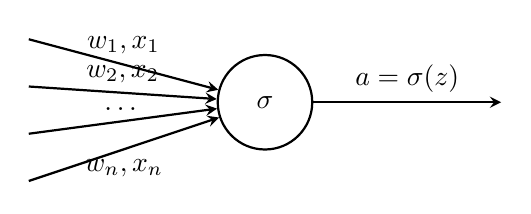
\begin{tikzpicture}[>=stealth,thick]
  \node[circle,draw,minimum size=1.2cm] (n) {$\sigma$};
  \draw[->] (-3,0.8) -- (n) node[midway,above] {$w_1,x_1$};
  \draw[->] (-3,0.2) -- (n) node[midway,above] {$w_2,x_2$};
  \draw[->] (-3,-0.4) -- (n) node[midway,above] {$\dots$};
  \draw[->] (-3,-1) -- (n) node[midway,below] {$w_n,x_n$};
  \draw[->] (n) -- (3,0) node[midway,above] {$a=\sigma(z)$};
\end{tikzpicture}

\end{frame}

%------------------------------------------------
% Page 2: Layers
\begin{frame}{Layers}

Suppose layer $0$ has activations $a^{(0)}_1,\dots,a^{(0)}_{N^{(0)}}$ 
and layer $1$ has pre-activations $z^{(1)}_1,\dots,z^{(1)}_{N^{(1)}}$ and
activations $a^{(1)}_j = \sigma(z^{(1)}_j)$.

\medskip

Let $W^{(1)}$ be the matrix of weights from layer $0$ to layer $1$,
with entries $w^{(1)}_{ij}$.

\[
  z^{(1)}_j = \sum_{i=1}^{N^{(0)}} a^{(0)}_i\,w^{(1)}_{ij},
  \qquad j=1,\dots,N^{(1)}.
\]

In vector / matrix form:
\[
  \bm{z}^{(1)} = \bm{a}^{(0)} W^{(1)}, \qquad
  \bm{a}^{(1)} = \sigma\!\left(\bm{z}^{(1)}\right),
\]
where $\sigma$ is applied elementwise.

\end{frame}

%------------------------------------------------
% Page 3: The feed-forward function
\begin{frame}{The Feed-forward Function of a Network}

With all weights specified, a network defines a function
(the \emph{feed-forward function})
\[
  F_{\bm{W}} : \text{inputs} \longrightarrow \text{outputs}.
\]

Example: three layers (input, hidden, output).

\medskip
Let
\[
  \bm{z}^{(0)} \in \mathbb{R}^{1\times 3},\quad
  W^{(1)} \in \mathbb{R}^{3\times 2},\quad
  W^{(2)} \in \mathbb{R}^{2\times 3}.
\]

Then
\[
  \bm{z}^{(1)} = \bm{z}^{(0)} W^{(1)}, \qquad
  \bm{a}^{(1)} = \sigma(\bm{z}^{(1)}),
\]
\[
  \bm{z}^{(2)} = \bm{a}^{(1)} W^{(2)}, \qquad
  \bm{a}^{(2)} = \sigma(\bm{z}^{(2)}).
\]

Thus the overall map is
\[
  F_{\bm{W}}(\bm{z}^{(0)}) = \sigma\!\bigl(\sigma(\bm{z}^{(0)} W^{(1)}) W^{(2)}\bigr),
\]
a composition of affine maps and elementwise nonlinearities.

\end{frame}

%------------------------------------------------
% Page 4: Linear regression
\begin{frame}{Linear Regression as a Neural Network}

Let
\[
  \bm{x} \in \mathbb{R}^{1\times N},\qquad
  W^{(1)} \in \mathbb{R}^{N\times M}.
\]

No hidden layer, no nonlinearity:
\[
  \hat{\bm{y}} = \bm{x} W^{(1)}.
\]

This is exactly a \emph{linear regression} model with
\[
  \hat{y}_j = \sum_{i=1}^N x_i w^{(1)}_{ij},
  \quad 1 \le j \le M.
\]

So linear regression can be seen as a one-layer neural network with
identity activation.

\end{frame}

%------------------------------------------------
% Page 5: Logistic / softmax regression
\begin{frame}{Logistic / Softmax Regression}

Again let $\bm{x} \in \mathbb{R}^{1\times N}$ and
$W^{(1)} \in \mathbb{R}^{N\times M}$.

Compute the logits
\[
  \bm{z}^{(1)} = \bm{x} W^{(1)}.
\]

For multi-class classification we apply the \emph{softmax}:
\[
  \hat{y}_j
   = \operatorname{softmax}(\bm{z}^{(1)})_j
   = \frac{e^{z^{(1)}_j}}{\sum_{k=1}^M e^{z^{(1)}_k}},
  \qquad j=1,\dots,M.
\]

This model is (multi-class) logistic regression written in neural-network
notation.

\end{frame}

%------------------------------------------------
% Page 6: A hidden layer
\begin{frame}{A Network with a Hidden Layer}

Let $N^{(0)}$ be the number of inputs, $N^{(1)}$ the size of a hidden
layer, and $N^{(2)}$ the number of outputs.

\medskip

Weights:
\[
  W^{(1)} \in \mathbb{R}^{N^{(0)}\times N^{(1)}},\qquad
  W^{(2)} \in \mathbb{R}^{N^{(1)}\times N^{(2)}}.
\]

Forward propagation:
\[
  \bm{z}^{(1)} = \bm{x} W^{(1)}, \qquad
  \bm{a}^{(1)} = \sigma(\bm{z}^{(1)}),
\]
\[
  \bm{z}^{(2)} = \bm{a}^{(1)} W^{(2)}, \qquad
  \bm{a}^{(2)} = \sigma(\bm{z}^{(2)}) \quad\text{(or softmax at output).}
\]

Such networks can represent much more complex functions than linear
models.

\end{frame}

%------------------------------------------------
% Page 7: Training and loss
\begin{frame}{Training a Network}

Given a network $F_{\bm{W}}$ depending on weights $\bm{W}$:

\begin{itemize}
  \item Data: $(\bm{x}^{(i)}, \bm{y}^{(i)})$, for $i=1,\dots,M$.
  \item Loss for example $i$:
        $L\bigl(\bm{y}^{(i)}, F_{\bm{W}}(\bm{x}^{(i)})\bigr)$.
\end{itemize}

The \emph{empirical loss} is
\[
  \mathcal{L}(\bm{W})
   = \frac{1}{M}\sum_{i=1}^M
     L\bigl(\bm{y}^{(i)}, F_{\bm{W}}(\bm{x}^{(i)})\bigr).
\]

\medskip

\textbf{Important:} $\mathcal{L}$ is a function of the \emph{weights} $\bm{W}$;
the data $\{(\bm{x}^{(i)},\bm{y}^{(i)})\}$ is fixed.

\medskip

\textbf{Goal:} Minimize $\mathcal{L}(\bm{W})$ by adjusting $\bm{W}$.

\end{frame}

%------------------------------------------------
\begin{frame}{Gradient Descent}

For each layer $\ell$ we have a weight matrix $W^{(\ell)}$ with entries
$w^{(\ell)}_{ij}$.

\medskip

Gradient descent updates:
\[
  w^{(\ell)}_{ij} \leftarrow
  w^{(\ell)}_{ij}
  - \eta \,\frac{\partial \mathcal{L}}{\partial w^{(\ell)}_{ij}},
\]
where $\eta>0$ is the learning rate.

\medskip

The main computational task is to compute the derivatives
$\frac{\partial \mathcal{L}}{\partial w^{(\ell)}_{ij}}$ efficiently for
all weights.  This is what \emph{backpropagation} does.

\end{frame}

%------------------------------------------------
% Pages 8–9: Backprop output layer
\begin{frame}{Backpropagation: Output Layer}

Backpropagation computes the gradients
$\frac{\partial \mathcal{L}}{\partial w^{(\ell)}_{ij}}$
efficiently using the network's graph structure.

\medskip

Let the output layer have pre-activations
$\bm{z}^{(L)}$ and outputs $\bm{a}^{(L)}$.

Define
\[
  \delta^{(L)}_j
      = \frac{\partial \mathcal{L}}{\partial z^{(L)}_j}.
\]

\textbf{Examples of $\delta^{(L)}$:}

\begin{itemize}
  \item \textbf{Mean squared error (MSE):}
    \[
      L(\bm{y},\bm{z}) = \frac{1}{2}\sum_j (y_j - z_j)^2
      \quad\Rightarrow\quad
      \delta^{(L)}_j = z^{(L)}_j - y_j.
    \]
  \item \textbf{Softmax + cross-entropy:}
    \[
      p_j = \frac{e^{z^{(L)}_j}}{\sum_k e^{z^{(L)}_k}},\qquad
      L(\bm{y},\bm{z}) = -\sum_j y_j \log p_j,
    \]
    then
    \[
      \delta^{(L)}_j = p_j - y_j.
    \]
\end{itemize}

\end{frame}

%------------------------------------------------
% Page 10: Earlier layers
\begin{frame}{Backpropagation: Earlier Layers}

For a hidden layer $\ell$ with pre-activations $\bm{z}^{(\ell)}$,
activations $\bm{a}^{(\ell)} = \sigma(\bm{z}^{(\ell)})$, and weight
matrix $W^{(\ell+1)}$ from layer $\ell$ to $\ell+1$:

\medskip

Define
\[
  \delta^{(\ell)}_j
    = \frac{\partial \mathcal{L}}{\partial z^{(\ell)}_j}.
\]

Using the chain rule one obtains the recursion
\[
  \bm{\delta}^{(\ell)}
   = \bigl(\bm{\delta}^{(\ell+1)} (W^{(\ell+1)})^\top\bigr)
      \;\odot\;
      \sigma'\!\left(\bm{z}^{(\ell)}\right),
\]
where $\odot$ denotes elementwise (Hadamard) product and $\sigma'$ is the
derivative of $\sigma$ applied elementwise.

\end{frame}

%------------------------------------------------
% Page 11: Gradients w.r.t. weights
\begin{frame}{Gradients with Respect to the Weights}

For the connection from layer $\ell-1$ to layer $\ell$:

\[
  z^{(\ell)}_j = \sum_i a^{(\ell-1)}_i w^{(\ell)}_{ij},
  \qquad
  a^{(\ell)}_j = \sigma(z^{(\ell)}_j).
\]

By the chain rule
\[
  \frac{\partial \mathcal{L}}{\partial w^{(\ell)}_{ij}}
   = a^{(\ell-1)}_i\,\delta^{(\ell)}_j.
\]

\medskip

In matrix form, letting
$\bm{a}^{(\ell-1)}$ be a row vector and $\bm{\delta}^{(\ell)}$ a row
vector,
\[
  \frac{\partial \mathcal{L}}{\partial W^{(\ell)}}
   = (\bm{a}^{(\ell-1)})^\top \bm{\delta}^{(\ell)},
\]
the outer product of the previous activations and current layer errors.

\end{frame}

%------------------------------------------------
% Page 12: Practical backprop steps
\begin{frame}{Backpropagation in Practice}

To exploit these formulas:

\begin{enumerate}
  \item During the \textbf{forward pass}, for each layer:
    \begin{itemize}
      \item compute and store $\bm{z}^{(\ell)}$,
      \item compute and store $\bm{a}^{(\ell)} = \sigma(\bm{z}^{(\ell)})$.
    \end{itemize}
  \item During the \textbf{backward pass}:
    \begin{itemize}
      \item compute $\bm{\delta}^{(L)}$ at the output layer,
      \item propagate backward using
        $\bm{\delta}^{(\ell)} =
           (\bm{\delta}^{(\ell+1)} (W^{(\ell+1)})^\top)
           \odot \sigma'(\bm{z}^{(\ell)})$,
      \item compute
        $\frac{\partial \mathcal{L}}{\partial W^{(\ell)}}
           = (\bm{a}^{(\ell-1)})^\top \bm{\delta}^{(\ell)}$.
    \end{itemize}
\end{enumerate}

Gradients over a dataset are obtained by summing / averaging the
contributions from each training example.

\end{frame}

%------------------------------------------------
% Page 13: Training algorithm / epoch
\begin{frame}{Training Algorithm (One Epoch)}

\textbf{Initialize:}
\begin{itemize}
  \item Initialize weights $W^{(\ell)}$ randomly (e.g.\ small Gaussian).
  \item Biases (if present) may be initialized to zero.
\end{itemize}

\medskip

\textbf{For each training example $(\bm{x}^{(i)},\bm{y}^{(i)})$:}

\begin{enumerate}
  \item \textbf{Forward pass:}
    compute and store all $\bm{z}^{(\ell)}$, $\bm{a}^{(\ell)}$.
  \item \textbf{Backward pass:}
    compute $\bm{\delta}^{(\ell)}$ for all layers and the gradients
    $\frac{\partial \mathcal{L}}{\partial W^{(\ell)}}$.
  \item \textbf{Update:}
    \[
      W^{(\ell)} \leftarrow
      W^{(\ell)} - \eta
      \,\frac{\partial \mathcal{L}}{\partial W^{(\ell)}}
      \quad\text{(possibly using mini-batches)}.
    \]
\end{enumerate}

One full pass through the dataset is a \emph{training epoch}.
Repeat epochs until the loss stops decreasing (or another stopping
criterion is met).

\end{frame}

%------------------------------------------------
\end{document}
